%
% Report -- Verilog-A compact device models for GaAs MESFETs
%
% Copyright (C) 2008 Mike Brinson <mbrin72043@yahoo.co.uk>
%
% Permission is granted to copy, distribute and/or modify this document
% under the terms of the GNU Free Documentation License, Version 1.1
% or any later version published by the Free Software Foundation.
%

% redefine subfigure caption
\renewcommand{\thesubfigure}{\thefigure(\alph{subfigure})}
\makeatletter
  \renewcommand{\@thesubfigure}{\thesubfigure:\space}
  \renewcommand{\p@subfigure}{}
\makeatother

% redefine subtable caption
\renewcommand{\thesubtable}{\thetable(\alph{subtable})}
\makeatletter
  \renewcommand{\@thesubtable}{\thesubtable:\space}
  \renewcommand{\p@subtable}{}
\makeatother

\tutsection{Introduction}

A previous Qucs Report\footnote{M. Brinson and S. Jahn, Qucs: Compact
device- circuit macromodel specification; A Curtice level 1 MESFET
model, http://qucs.sourceforge.net/docs.html} described a MESFET model
based on an equation defined device (EDD) representation of the level
1 Curtice model. This model evolved as a test example during the
initial Qucs EDD development phase. Today the EDD model is popular
amongst Qucs users as either a powerful non-linear component in it's
own right or as the basis of a component prototyping system for
constructing compact Verilog-A device models, translated with ADMS to
C++ code, compiled to object code and finally linked to the main body
of the Qucs program code. Over the last year the Qucs development team
has invested a significant amount of time improving both EDD
prototyping and Verilog-A compact device/circuit model development,
making the development process more transparent to anyone interested
in trying their hand at model construction. One branch of the current
Qucs modelling activities is concentrating on adding new models which
fill in some of the gaps in the Qucs released model lists. One such
model in this category is the GaAs MESFET. This report outlines the
background and mathematical basis for a number of MESFET models. These
have been coded in Verilog-A and tested using recent Qucs CVS
code. They will be included in the next full release of Qucs.

\tutsection{The GaAs MESFET}

The metal-semiconductor FET (MESFET) is a Schottky-barrier gate FET
which is normally made from Gallium Arsenide.  It is a popular device
for high frequency applications because of it's high electron mobility
and usable gain at microwave frequencies. An early simulation model
for the MESFET device was developed by Walter
R. Curtice\footnote{W.R. Curtice, 1980, A MESFET model for use in the
design of GaAs integrated circuits, IEEE Transactions on Microwave
Theory and Techniques, MTT-28, pp. 448-456.} in 1980 at the RCA
Laboratory in Princeton, New Jersey, USA. Since Curtice published his
original MEFET model a number of authors have contributed improvements
to the basic model, including for example Statz
\textit{et. al}. (Raytheon)\footnote{H. Statz, P. Newman, I.W. Smith,
R.A. Pucel, and H.A. Haus, gaAs FET Device and Circuit Simulation in
SPICE, IEEE Transactions on Electron Devices, Vol. 34, pp. 160-169,
Feb. 1987.} and TriQuint Semiconductor Inc.\footnote{For example,
D.H. Smith, TOM-2: An improved Model for GaAs MESFETs, TriQuint
Report, TriQuint Semiconductor, Inc Fe. 27, 1995 (11 pages).}. These
models form the basis of the Qucs MESFET model described in this
report.

\tutsection{The Qucs MESFET model}

Parameters
\begin{longtable}{rllll}
Name & Symbol & Description & Unit & Default\\
\hline
\endhead
LEVEL &          & model selector                        &                   & $1$\\
Vto   & $V_{to}$ & gate threshold voltage                & $\volt$           & $-1.8$\\
Beta  & $\beta$  & transconductance parameter            & $\ampere/\volt^2$ & $3\milli$\\
Alpha & $\alpha$ & coefficient of Vds in tanh function   & $1/\volt$         & $2.25$\\
Gamma & $\gamma$ & dc drain pull coefficient             &                   & $0.015$\\
Lambda & $\lambda$ & channel length modulation parameter & $1/\volt$         & $0.05$\\
B      & $B$       & doping profile parameter            & $1/\volt$         & $0$\\
Qp     & $Qp$      & power law exponent parameter       &                   & $2.1$\\
Delta  & $\delta$  & power feedback parameter            & $1/\watt$         & $0.1$\\
Vmax   & $Vmax$    & \parbox[t]{5.5cm}{maximum junction voltage before cap. limiting} & $\volt$ & $0.5$\\
Vdelta1 & $Vdelta1$ & \parbox[t]{5.5cm}{capacitance saturation transition voltage} & $\volt$ & $0.3$\\
Vdelta2 & $Vdelta2$ & \parbox[t]{5.5cm}{capacitance threshold transition voltage}  & $\volt$ & $0.2$\\
Nsc     & $Nsc$     & subthreshold conductance parameter          &          & $1$\\
Is & $I_{S}$ & diode saturation current   & $\ampere$ & $10\femto$\\ 
N  & $N$     & diode emission coefficient &           &  $1$\\
Vbi& $Vbi$   & built-in gate potential   & $\volt$  & $1.0$\\
Bv & $Bv$    & diode breakdown voltage  & $\volt$ & $60$\\
XTI & $X_{TI}$ & \parbox[t]{5.5cm}{diode saturation current temperature coefficient} &   & $0$\\
TAU & $\tau$ & \parbox[t]{5.5cm}{internal time delay from drain to source} & $\second$ & $10\pico$\\
Rin & $Rin$ & series resistance to Cgs & $\ohm$ & $1\milli$\\
Fc  & $Fc$   & \parbox[t]{5.5cm}{forward-bias depletion capacitance coefficient} &     & $0.5$\\
Area & $Area$& area factor & & $1$\\
Eg   & $Eg$  & bandgap voltage    &  $\volt$ & $1.11$\\
M    & $M$   & grading coefficient &         & $0.5$\\
Cgs & $Cgs$ & zero-bias gate-source capacitance & $\farad$ & $0.2\pico$\\
Cgd & $Cgd$ & zero-bias gate-drain capacitance & $\farad$ & $1\pico$\\
Cds & $Cds$ & zero-bias drain-source capacitance & $\farad$ & $1\pico$\\
Betatc & $Betatc$ & Beta temperature coefficient  & $\%/\Celsius$ & $0$\\
Alphatc & $Alphatc$ & Alpha temperature coefficient  & $\%/\Celsius$ & $0$\\
Gammatc & $Gammatc$ & Gamma temperature coefficient  & $\%/\Celsius$ & $0$\\
Ng      & $Ng$      & subthreshold slope gate parameter &    & $2.65$\\
Nd      & $Nd$      & subthreshold drain pull parameter &    & $-0.19$\\
ILEVELS & $ILEVELS$ & gate-source current equation selector &   & $3$\\
ILEVELD & $ILEVELD$ & drain-source current equation selector &   & $3$\\ 
QLEVELS & $QLEVELS$ & gate-source charge equation selector &   & $2$\\
QLEVELD & $QLEVELS$ & gate-source charge equation selector &   & $2$\\
QLEVELDS & $QLEVELDS$ & drain-source charge equation selector &   & $2$\\
Vtotc    & $Vtotc$    & Vto temperature coefficient &  $\volt/\Celsius$ & $0$\\
Rg & $Rg$ & gate series resistance & $\ohm$ & $5.1$\\
Rd & $Rd$ & drain series resistance & $\ohm$ & $1.3$\\
Rs & $Rs$ & source series resistance & $\ohm$ & $1.3$\\
Rgtc & $Rgtc$ & \parbox[t]{5.5cm}{gate series resistance temperature coefficient} & $1/\Celsius$ & $0$\\
Rdtc & $Rdtc$ & \parbox[t]{5.5cm}{drain series resistance temperature coefficient} & $1/\Celsius$ & $0$\\
Rstc & $Rstc$ & \parbox[t]{5.5cm}{source series resistance temperature coefficient} & $1/\Celsius$ & $0$\\
Ibv  & $Ibv$  & gate reverse breakdown current & $\ampere$  & $1\milli$\\
Rf   & $Rf$   & forward bias slope resistance & $\ohm$  & $10$\\
R1   & $R1$   & breakdown slope resistance    & $\ohm$  & $10$\\
Af   & $Af$   & Flicker noise exponent        &         & $1.0$\\
Kf   & $Kf$   & flicker noise coefficient     &         & $0.0$\\
Gdsnoi & $Gdnsnoi$ & shot noise coefficient   &         & $1.0$\\
Tnom & $Tnom$ & \parbox[t]{5.5cm}{device parameter measurement temperature} & $\celsius$ & $26.85$\\
Temp & $Temp$ & device circuit temperature & $\celsius$ & $26.85$\\


\end{longtable}

Where parameter LEVEL selects a MESFET model listed in Table~\ref{tab:tab3}.

\begin{table} [here]
\begin{center}
% use packages: array
\newcommand{\mc}[3]{\multicolumn{#1}{#2}{#3}}
%
\begin{tabular}{ll}
LEVEL & MESFET model type \\ 
\mc{1}{c}{1} & Quadratic Curtice - basic form \\ 
\mc{1}{c}{2} & Quadratic Curtice - basic plus subthreshold properties \\ 
\mc{1}{c}{3} & Statz et. al. (Raytheon)  - same as SPICE 3f5 \\ 
\mc{1}{c}{4} & TriQuint  - TOM 1 model \\ 
\mc{1}{c}{5} & TriQuint  -  TOM 2 model
\end{tabular}
\caption{Qucs MESFET model types}
\label{tab:tab3} 
\end{center}
\end{table}

MESFET gate current equations can be selected by setting parameters
ILEVELS and ILEVELD.  Table~\ref{tab:tab4} lists the available
options.

\begin{table} [here]
\begin{center}
% use packages: array
\newcommand{\mc}[3]{\multicolumn{#1}{#2}{#3}}
%
\begin{tabular}{lll}
\mc{1}{c}{ILEVELS - ILEVELD} & \mc{1}{c}{Gate-source current} & \mc{1}{c}{Gate-drain current} \\ 
\mc{1}{c}{0} & Igs=0 & Igd=0 \\ 
\mc{1}{c}{1} & Linear no reverse breakdown & Linear no reverse breakdown \\ 
\mc{1}{c}{2} & Linear with reverse breakdown & Linear with reverse breakdown \\ 
\mc{1}{c}{3} & Diode no reverse breakdown & Diode  no reverse breakdown \\ 
\mc{1}{c}{4} & Diode with reverse breakdown & Diode with reverse breakdown
\end{tabular}
\caption{Qucs MESFET gate current model types}
\label{tab:tab4}
\end{center}
\end{table}

MESFET charge equations can be selected by setting parameters QLEVELS,
QLEVELD and QLEVELDS.  Table~\ref{tab:tab5} lists the available
options. Although it is possible to mix the five basic MESFET models
with different gate current and charge equation models the common
default models are the ones listed in Table~\ref{tab:tab6}.

\begin{table} [here]
\begin{center}
% use packages: array
\newcommand{\mc}[3]{\multicolumn{#1}{#2}{#3}}
%
\begin{tabular}{llllll}
\mc{1}{c}{QLEVELS} &  & \mc{1}{c}{QLEVELD} &   & \mc{1}{c}{QLEVELDS} &   \\ 
\mc{1}{c}{0} & Qgs=0 & \mc{1}{c}{0} & Qgd=0 & \mc{1}{c}{0} & Qds=0 \\ 
\mc{1}{c}{1} & Constant cap. & \mc{1}{c}{1} & Constant cap. & \mc{1}{c}{1} & Constant cap. \\ 
\mc{1}{c}{2} & Diode & \mc{1}{c}{2} & Diode  & \mc{1}{c}{2} & Constant cap.+ transit \\ 
\mc{1}{c}{3} & Statz & \mc{1}{c}{3} & Statz  &              &  
\end{tabular}
\caption{Qucs MESFET charge equation types}
\label{tab:tab5}
\end{center}
\end{table}

\begin{table} [here]
\begin{center}
% use packages: array
\newcommand{\mc}[3]{\multicolumn{#1}{#2}{#3}}
%
\begin{tabular}{lllllll}
Model & LEVEL & ILEVELS & ILEVELD & QLEVELS & QLEVELD & QLEVELDS \\ 
Curtice L1 & \mc{1}{c}{1} & \mc{1}{c}{0 to 4} & \mc{1}{c}{0 to 4} & \mc{1}{c}{0 to 2} & \mc{1}{c}{0 to 2} & \mc{1}{c}{0 to 2} \\ 
Curtice (Adv.) & \mc{1}{c}{2} & \mc{1}{c}{0 to 4} & \mc{1}{c}{0 to 4} & \mc{1}{c}{0 to 2} & \mc{1}{c}{0 to 2} & \mc{1}{c}{0 to 2} \\ 
Statz-Raytheon & \mc{1}{c}{3} & \mc{1}{c}{4} & \mc{1}{c}{4} & \mc{1}{c}{3} & \mc{1}{c}{3} & \mc{1}{c}{2} \\ 
TOM 1 & \mc{1}{c}{4} & \mc{1}{c}{4} & \mc{1}{c}{4} & \mc{1}{c}{3} & \mc{1}{c}{3} & \mc{1}{c}{2} \\ 
TOM 2 & \mc{1}{c}{5} & \mc{1}{c}{4} & \mc{1}{c}{4} & \mc{1}{c}{3} & \mc{1}{c}{3} & \mc{1}{c}{2}
\end{tabular}
\caption{Qucs MESET default selection parameters}
\label{tab:tab6}
\end{center}
\end{table} 
 
\tutsection{The Qucs MESFET simulation model}

The large signal equivalent circuit for the Qucs MESFET model is
illustrated in Fig.~\ref{fig:fig1}. The currents flowing in each of
the circuit branches are given by the Verilog-A code fragment shown in
Fig.~\ref{fig:fig1}. The Verilog-A HDL code for the entire Qucs MESFET
model is available from the Qucs CVS
archive\footnote{http://qucs.sourceforge.net/}.  In order to simulate
the operation of an MESFET, equations based on the physical operation
of the device are required for all the current contribution components
in Fig.~\ref{fig:fig1}. These equations are presented in the remaining
sections of this report.  Examples are also introduced to demonstrate
the simulation performance of each model.


\tutsection{MESFET gate current equations}

\begin{itemize}
 \item ILEVELS = 0: $Igs = 0$ A
 \item ILEVELS = 1: 
if $(V(b1)>Vbi)$ 
\begin{equation} Igs = \dfrac{V(b1)-Vbi}{Rf}  \end{equation}
else \hspace{50mm} $Igs = -Area \cdot Is +GMIN \cdot V(b1)$ 
 \item ILEVELS = 2: 
if $(V(b1) > Vbi)$
\begin{equation} Igs1 = \dfrac{V(b1)-Vbi}{Rf}  \end{equation}
else \hspace{50mm}$Igs1 = -Area \cdot Is +GMIN \cdot V(b1)$


if $V(b1) < -Bv)$
\begin{equation} Igs2 = \dfrac{V(b1)-Vbi}{R1}  \end{equation}
\begin{equation} Igs = Igs1 + Igs2  \end{equation}
 \item  ILEVELS = 3: 
if $(V(b1) >Vbi) $
\begin{equation} Igs = Is\_T2 \cdot \left\lbrace  limexp\left(  \frac{V(b1)}{N \cdot Vt\_T2}\right) -1.0\right\rbrace   + GMIN \cdot V(b1)   \end{equation}
else \hspace{13mm}$Igs = -Is\_T2 + GMIN\cdot V(b1)$ 

 \item  ILEVELS = 4: 
if $(V(b1) > -5 \cdot N \cdot Vt\_T2)$
\begin{equation} 
Igs1 = Area \cdot Is\_T2 \cdot \left\lbrace limexp\left( \frac{V(b1)}{N \cdot Vt\_T2}\right)  -1.0 \right\rbrace  + GMIN \cdot V(b1)
 \end{equation}
 else \hspace{5mm} $Igs1 = 0$


if $( (-Bv < V(b1)) $ and $ (V(b1) < -5\cdot N \cdot Vt\_T2))$
\begin{equation} Igs2 = -Area \cdot Is\_T2 + GMIN \cdot V(b1)  \end{equation}
else  \hspace{31mm}$Igs2 = 0$


if $(V(b1) == -Bv)$
\begin{equation} Igs3 = -Ibv \end{equation}
else  \hspace{56mm}$Igs3 = 0$


if $(V(b1) < -Bv)$
\begin{equation} Igs4 = -Area \cdot Is\_T2 \cdot \left\lbrace limexp\left( \frac{-(Bv+V(b1))}{Vt\_T2}\right)  -1.0 + \frac{Bv}{Vt\_T2}\right\rbrace  \end{equation}
else \hspace{5mm}$Igs4 = 0$
\begin{equation} Igs = Igs1 + Igs2 + Igs3 + Igs4  \end{equation}
\end{itemize}

Where xx\_T2 indicates the values of temperature dependent parameters
at circuit temperature T2.  See later sections of this report for more
details.  The gate to drain current equations are identical except Igs
is replaced by Igd, Igsx by Igdx, and V(b1) by V(b2). More details can
be found in the Verilog-A listing given in the Qucs CVS code held at
the Qucs Sourceforge site.
\begin{figure} 
  \centering
  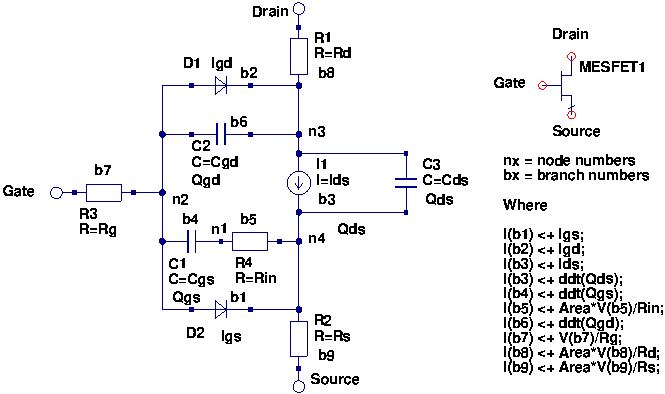
\includegraphics[width=0.9\linewidth]{MESFET_Fig1}
  \caption{Qucs MESFET symbol and large signal equivalent circuit} 
  \label{fig:fig1}
\end{figure}

\tutsection{MESFET charge equations QLEVELS 0 to 2}
\begin{itemize}
 \item QLEVELS = 0: [NO charge]:

\begin{equation} Qgs = 0  \end{equation}
 \item QLEVELS = 1: [Fixed capacitor charge] 
\begin{equation} Qgs = Area \cdot Cgs \cdot V(b4) \end{equation}
 \item QLEVELS = 2: [Diode charge]

if $( V(b4) < (Fc \cdot Vbi) )$
\begin{equation} Qgs1 = \dfrac{Cgs\_T2 \cdot Vbi\_T2}{(1-M)} \cdot \left\lbrace 1 - \left( 1-\dfrac{V(b4)}{Vbi\_T2}\right) ^{1-M} \right\rbrace \end{equation}
\end{itemize}


\hspace{10mm} if $( V(b4) >= (Fc \cdot Vbi) )$

\begin{equation}
H1 =\dfrac{M}{2 \cdot Vbi\_T2}  \cdot \left( V(b4) \cdot V(b4) - \left( Fc \cdot Fc \cdot Vbi\_T2 \cdot Vbi\_T2 \right)  \right)
\end{equation}

\begin{equation} 
Qgs2 = Cgs\_T2 \cdot \left[ F1+\dfrac{1}{F2} \cdot \left\lbrace  F3 \cdot \left(  V(b4) - Fc \cdot Vbi\_T2 \right) +  H1  \right\rbrace  \right]
\end{equation}
 
Where,
\begin{align}
F1 &= \dfrac{Vbi\_T2}{1-M} \cdot \left\lbrace 1- \left(1-Fc\right) ^{1-M} \right\rbrace ,\\
F2 &= \left( 1-Fc\right) ^{1+M},
\end{align}
and 
\begin{align}
F3 &= 1-Fc \cdot \left( 1+M\right).
\end{align}

Again xx\_T2 indicates the values of temperature dependent parameters
at circuit temperature T2.  See a later section of this report for
more details.  The gate to drain charge equations (types 0 to 2) are
identical except Qgs is replaced by Qgd, Qgsx by Qgdx, and V(b4) by
V(b6). More details can be found in the Qucs CVS code held at the Qucs
Sourceforge site.

\tutsection{MESFET charge equations QLEVELDS 0 to 2}
\begin{itemize}
 \item QLEVELDS = 0: [NO charge]: \begin{equation} Qds = 0  \end{equation}
 \item QLEVELDS = 1: [Fixed capacitor charge]  \begin{equation} Qds = Area \cdot Cds \cdot V(b3) \end{equation}
 \item QLEVELS = 2: [Fixed capacitor plus transit charge] \begin{equation} Qds = Area \cdot Cds \cdot V(b3) + Tau \cdot Ids \end{equation}
\end{itemize}



\tutsection{Curtice hyperbolic tangent model: LEVEL = 1}

if $ (V(b1) - Vto\_T2) > 0$
\begin{equation}
 Ids = Beta\_T2 \cdot (V(b1)-Vto\_T2)^{2} \cdot \left\lbrace 1+Lambda \cdot V(b3) \right\rbrace  \cdot tanh(Alpha \cdot V(b3))
\end{equation} 

else $Ids = 0$.

\begin{figure} 
  \centering
  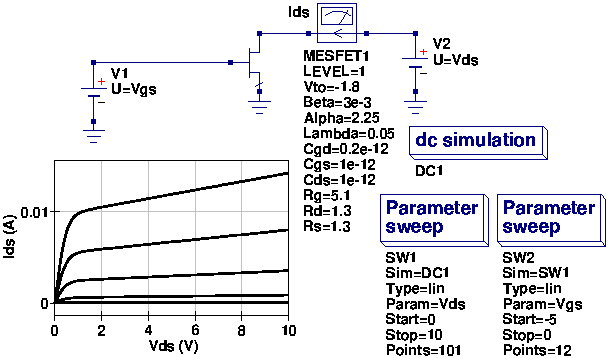
\includegraphics[width=0.9\linewidth]{MESFET_Fig2}
  \caption{Curtice LEVEL 1 DC test circuit and Ids-Vds characteristics}  
  \label{fig:fig2}
\end{figure}

\begin{figure} 
  \centering
  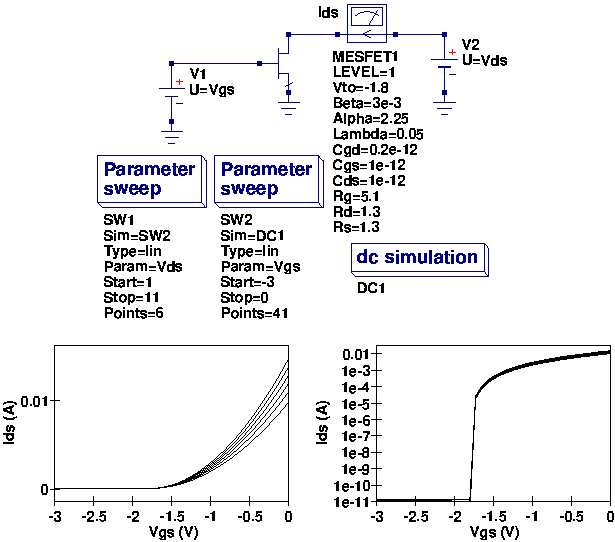
\includegraphics[width=0.9\linewidth]{MESFET_Fig3} 
  \caption{Curtice LEVEL 1 DC test circuit and Ids-Vgs characteristics} 
  \label{fig:fig3}
\end{figure} 

\begin{figure}
  \centering
  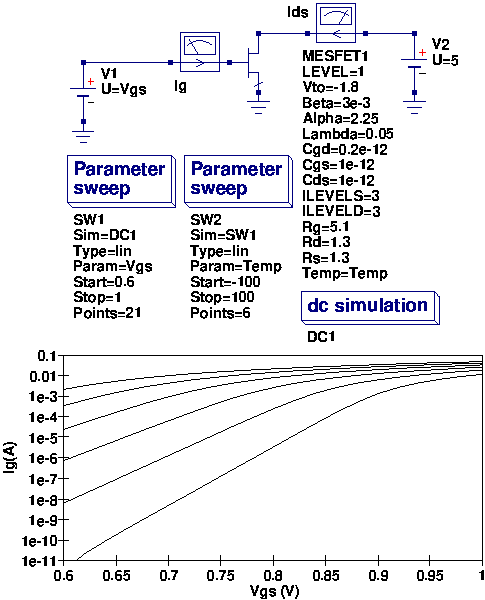
\includegraphics[width=0.9\linewidth]{MESFET_Fig4} 
  \caption{Curtice LEVEL 1 DC test circuit and Ig-Vgs characteristics} 
  \label{fig:fig4}
\end{figure} 

\begin{figure} 
  \centering
  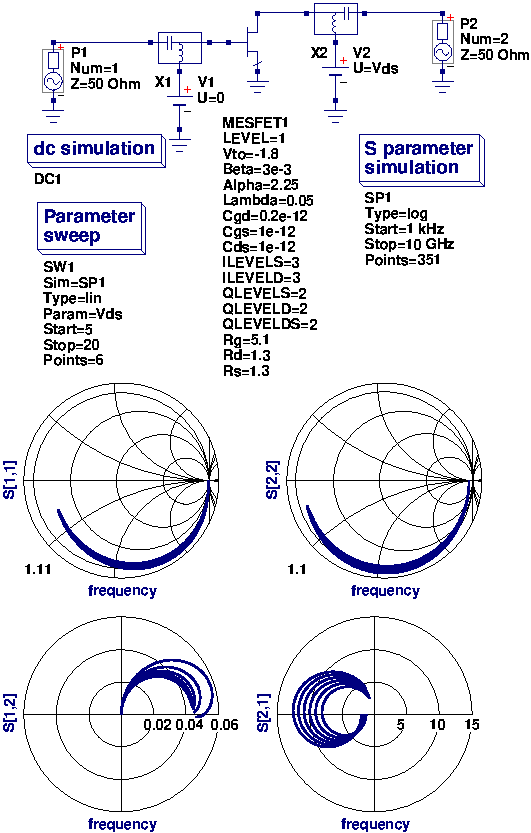
\includegraphics[width=0.9\linewidth]{MESFET_Fig5}
  \caption{Curtice LEVEL 1 S parameter test circuit and characteristics} 
  \label{fig:fig5}
\end{figure} 

\tutsection{Curtice hyperbolic tangent model with subthreshold modification: LEVEL = 2}
\begin{equation}
 Ids = Beta\_T2 \cdot Vf^{2} \cdot \left\lbrace 1+Lambda \cdot V(b3) \right\rbrace  \cdot tanh(Alpha \cdot V(b3))
\end{equation}  

Where
\begin{equation} Vf = \dfrac{1}{Ah}\cdot ln\left\lbrace 1+exp\left( Ah \cdot (V(b1)-Vto\_T2) \right) \right\rbrace 
 \end{equation} 

and
\begin{equation} Ah = \dfrac{1}{2 \cdot Nsc \cdot Vt\_T2}
 \end{equation}

When $V(b2) > Vto\_T2, Vf \Longrightarrow V(b2) - Vto\_T2$. Otherwise,
$Vf$ approaches zero asymptotically.  This modification to the basic
Curtice model provides an improved match to channel gradual pinch-off
and MESFET subthreshold conduction.

\begin{figure}  
  \centering
  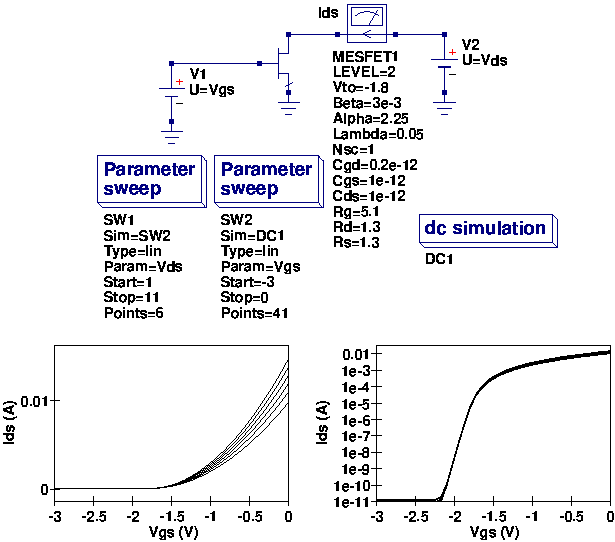
\includegraphics[width=0.9\linewidth]{MESFET_Fig6} 
  \caption{Curtice LEVEL 2 DC test circuit and Ids-Vgs characteristics illustrating subthreshold conduction modification} 
  \label{fig:fig6}
\end{figure} 

\tutsection{Statz \textit{et. al.} (Raytheon) model: LEVEL = 3}

if $ (V(b1) - Vto\_T2) > 0$


\hspace{5mm} if $( 0 < V(b3) ) $  and $( V(b3) < \dfrac{3}{Alpha} )$


\hspace{10mm}    begin
		\begin{equation}
 			H1 = \dfrac{1- \left\lbrace 1- \dfrac{Alpha \cdot V(b3)}{3}\right\rbrace ^{3}}{ 1+B \cdot (V(b1)-Vto\_T2) }
		\end{equation}
		\begin{equation}
 		Ids = Beta\_T2 \cdot \left\lbrace 1+Lambda \cdot V(b3) \right\rbrace \cdot  (V(b1)-Vto\_T2)^{2}  \cdot H1 
		\end{equation} 


\hspace{10mm}    end 

\hspace{5mm} if $( V(b3) > \dfrac{3}{Alpha} )$


                \begin{equation}
 		Ids = \dfrac{ Beta\_T2 \cdot \left\lbrace 1+Lambda \cdot V(b3) \right\rbrace \cdot  (V(b1)-Vto\_T2)^{2} } {1+B \cdot (V(b1) - Vto\_T2)} 
		\end{equation} 


else $Ids = 0$.

\begin{figure} 
  \centering
  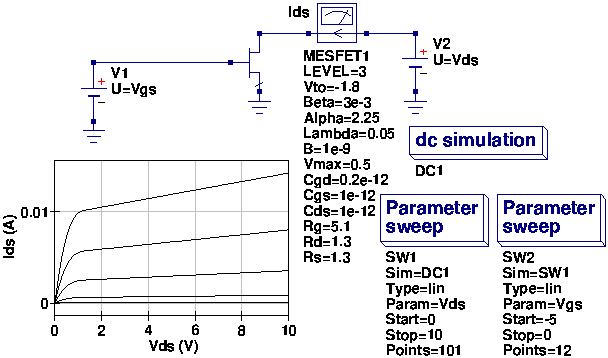
\includegraphics[width=0.9\linewidth]{MESFET_Fig7} 
  \caption{Statz \textit{et. al.} LEVEL 3 DC test circuit and Ids-Vds characteristics}  
  \label{fig:fig7}
\end{figure} 

\begin{figure} 
  \centering
  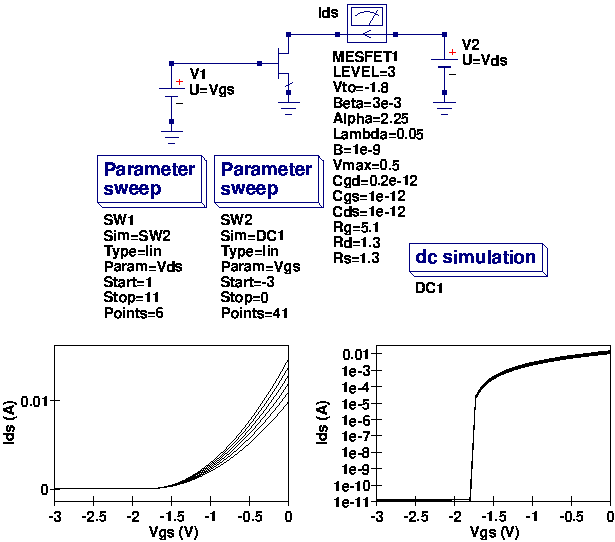
\includegraphics[width=0.9\linewidth]{MESFET_Fig8} 
  \caption{Statz \textit{et. al.} LEVEL 3 DC test circuit and Ids-Vgs characteristics} 
  \label{fig:fig8}
\end{figure} 

\begin{figure} 
  \centering
  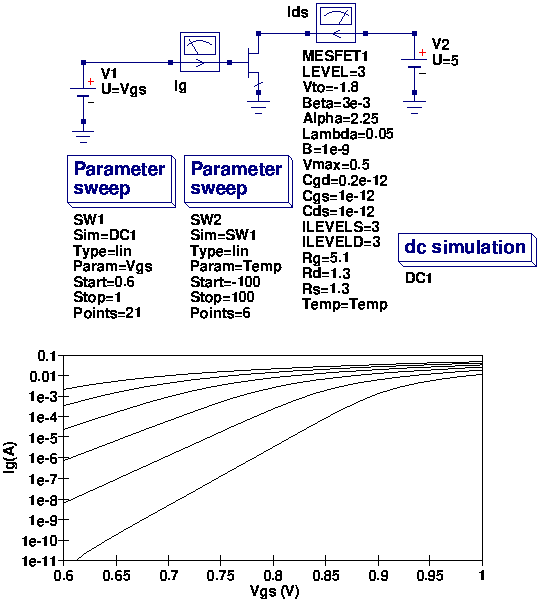
\includegraphics[width=0.9\linewidth]{MESFET_Fig9} 
  \caption{Statz\textit{ et. al.} LEVEL 3 DC test circuit and Ig-Vgs characteristics} 
  \label{fig:fig9}
\end{figure} 

\tutsubsection{MESFET charge equations QLEVELS = 3 and QLEVELD = 3}

QLEVELS = 3 : Statz et. al. charge equations
\begin{equation}
 Vmax = min(Fc \cdot Vbi, Vmax)
\end{equation}

\begin{equation}
 Veff1 = 0.5 \cdot \left\lbrace  V(b4)+V(b6)+\sqrt{ (V(b6)-V(b4))^{2} + Vdelta1^{2}  }\right\rbrace 
\end{equation}
\begin{equation}
 Vnew = 0.5 \cdot \left\lbrace Veff1 + Vto\_T2 + \sqrt{(Veff1-Vto\_T2)^{2} + Vdelta2^{2}} \right\rbrace 
\end{equation}

if $(Vnew > Vmax)$
	\begin{equation}
	 Qgs = Cgs\_T2 \cdot \left\lbrace 2 \cdot Vbi\_T2 \left( 1-\sqrt{1-\dfrac{Vmax}{Vbi\_T2}}\right) +\dfrac{Vnew-Vmax}{\sqrt{1-\dfrac{Vmax}{Vbi\_T2}}} \right\rbrace 
	\end{equation}
if $( Vnew <= Vmax )$
	\begin{equation}
	 Qgs = Cgs\_T2 \cdot 2 \cdot Vbi\_T2 \cdot \left\lbrace 1 - \sqrt{1-\dfrac{Vnew}{Vbi\_T2}} \right\rbrace 
	\end{equation}

QLEVELD = 3 : Statz et. al. charge equations

\begin{equation}
  Veff2 = 0.5 \cdot \left\lbrace V(b4) +V(b6) - \sqrt{(V(b4)-V(b6))^{2}+Vdelta1^{2}} \right\rbrace 
\end{equation}
\begin{equation}
  Qds = Cgd\_T2 \cdot Veff2
\end{equation}
During simulation gate charge must be partitioned between gate-source
and gate-drain branches. The Qucs implementation of the Statz
et. al. MESFET model uses the procedure adopted by Divehar
\footnote{D. Divehar, Comments on GaAs FET device and circuit
simulation in SPICE,IEEE Transactions on Electronic Devices,
Vol. ED-34, pp 2564-2565, Dec. 1987}.

\begin{figure} [here]
  \centering
  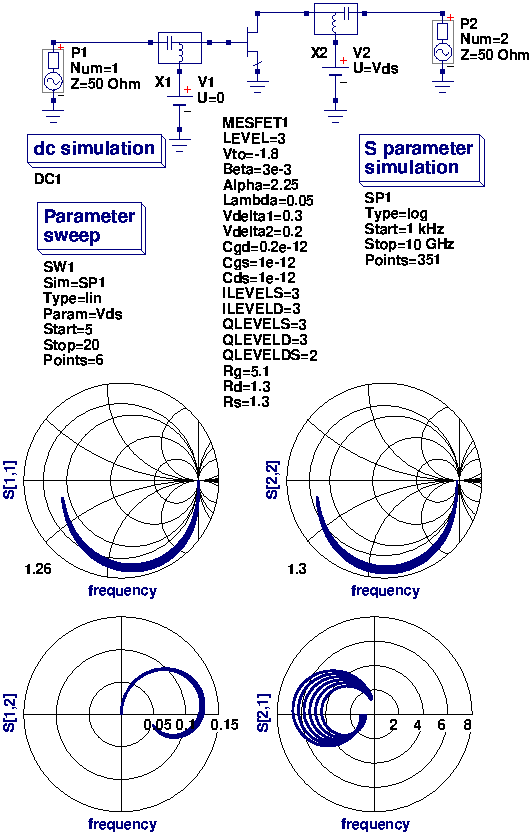
\includegraphics[width=0.9\linewidth]{MESFET_Fig10}  
  \caption{Statz\textit{ et. al.} LEVEL 3 S parameter test circuit and characteristics} 
  \label{fig:fig10}
\end{figure} 

\tutsection{TriQuint Semiconductor TOM 1 model: LEVEL = 4} 
if $ (V(b1) - Vto\_T2) > 0$


\hspace{5mm} if $( 0 < V(b3) ) $  and $( V(b3) < \dfrac{3}{Alpha} )$


\hspace{10mm}    begin
		\begin{equation}
		 	Ids1 = \left\lbrace Beta\_T2 \cdot \left( V(b1)-Vto\_T2\right) ^{Qp}\right\rbrace \cdot \left\lbrace 1- \left\lbrace 1- \dfrac{Alpha \cdot V(b3)}{3}\right\rbrace ^{3}\right\rbrace 
		\end{equation}		
		\begin{equation}
 		Ids = \dfrac{ Ids1 \cdot \left\lbrace 1+Lambda \cdot V(b3) \right\rbrace}{1+Delta \cdot V(b3) \cdot Ids1} 
		\end{equation} 


\hspace{10mm}    end 

\hspace{5mm} if $( V(b3) > \dfrac{3}{Alpha} )$
		\begin{equation}
		 	Ids1 = Beta\_T2 \cdot \left( V(b1)-Vto\_T2\right) ^{Qp}
		\end{equation}

                \begin{equation}
 		Ids = \dfrac{ Ids1 \cdot \left\lbrace 1+Lambda \cdot V(b3) \right\rbrace } {1+Delta \cdot (V(b3) \cdot Ids1} 
		\end{equation} 


else $Ids = 0$.
\begin{figure} 
  \centering
  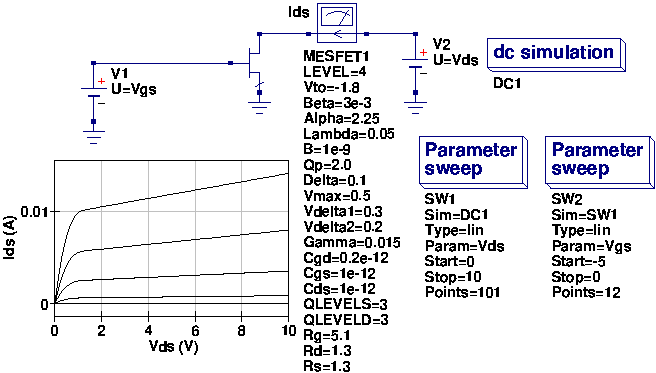
\includegraphics[width=0.9\linewidth]{MESFET_Fig11} 
  \caption{TOM1 LEVEL 4 DC test circuit and Ids-Vds characteristics}  
  \label{fig:fig11}
\end{figure} 

\begin{figure} 
  \centering
  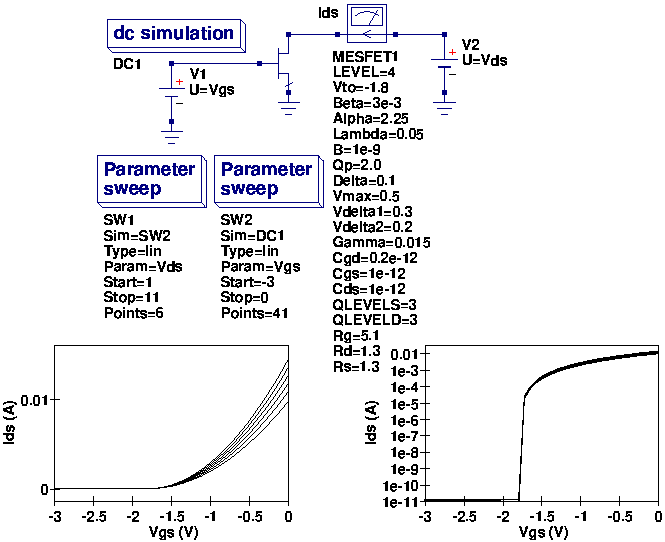
\includegraphics[width=0.9\linewidth]{MESFET_Fig12} 
  \caption{TOM1 LEVEL 4 DC test circuit and Ids-Vgs characteristics} 
  \label{fig:fig12}
\end{figure} 

\begin{figure} 
  \centering
  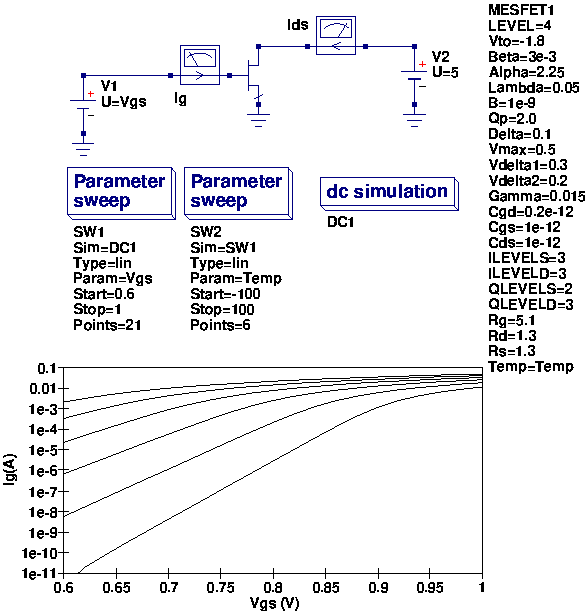
\includegraphics[width=0.9\linewidth]{MESFET_Fig13} 
  \caption{TOM1 LEVEL 4 DC test circuit and Ig-Vgs characteristics} 
  \label{fig:fig13}
\end{figure} 

\begin{figure} 
  \centering
  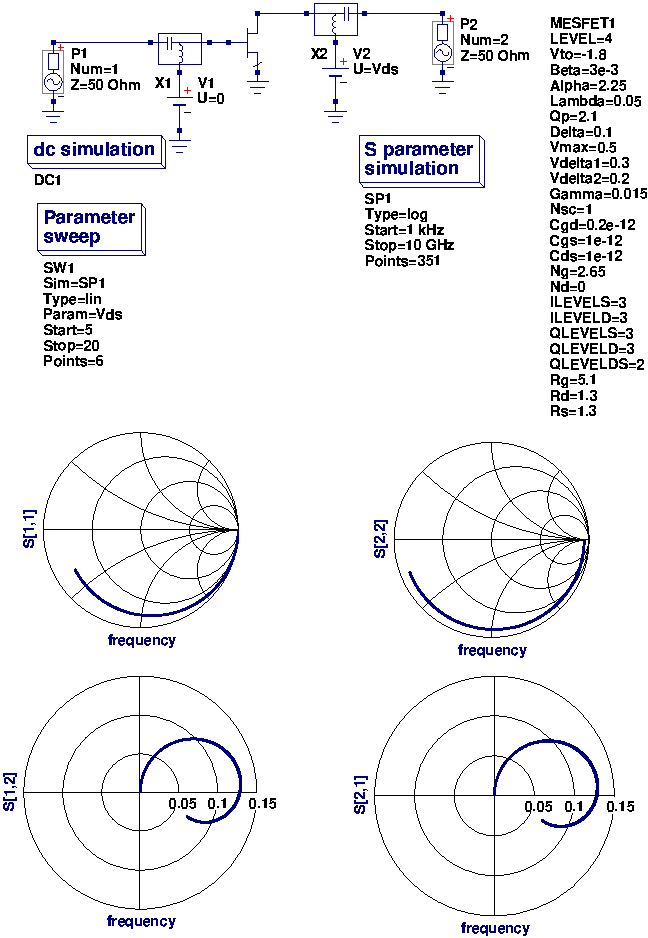
\includegraphics[width=0.9\linewidth]{MESFET_Fig14}  
  \caption{TOM1 LEVEL 4 S parameter test circuit and characteristics} 
  \label{fig:fig14}
\end{figure} 


\tutsection{TriQuint Semiconductor TOM 2 model: LEVEL = 5}
if $ (V(b1) - Vto\_T2) > 0$

\hspace{10mm}    begin
			\begin{equation}
			 	Nst = Ng + Nd \cdot V(b3)
			\end{equation}
\hspace{20mm} if $ (Nst < 1.0 ) Nst = 1.0$
			
			\begin{equation}
			Vst = Nst \cdot Vt\_T2 
			\end{equation}
			\begin{equation}
			 Vg = Qp \cdot Vst \cdot ln\left(  exp \left\lbrace \dfrac{V(b1)-Vto\_T2+Gamma\_T2 \cdot V(b3)}{Qp \cdot Vst} \right\rbrace +1 \right) 
			\end{equation}
			\begin{equation}
			 Al = Alpha\_T2 \cdot V(b3)
			\end{equation}
			\begin{equation}
			 Fd = \dfrac{Al}{\sqrt{1+Al \cdot Al}}
			\end{equation}
			\begin{equation}
			 Ids1 = Beta\_T2\cdot Vg^{Qp} \cdot Fd
			\end{equation}
			\begin{equation}
			 Ids = Ids1 \cdot \dfrac{1+Lambda \cdot V(b3)}{1+Delta \cdot V(b3) \cdot Ids1}
			\end{equation}
\hspace{10mm}    end


else $Ids =0$




\begin{figure}  
  \centering
  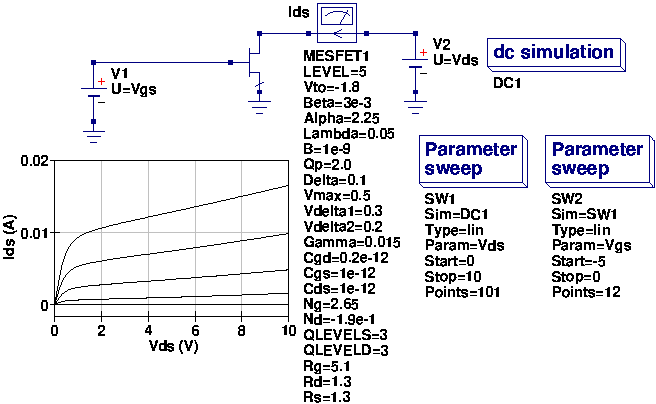
\includegraphics[width=0.9\linewidth]{MESFET_Fig15} 
  \caption{TOM2 LEVEL 5 DC test circuit and Ids-Vds characteristics}   
  \label{fig:fig15}
\end{figure}

\begin{figure} 
  \centering
  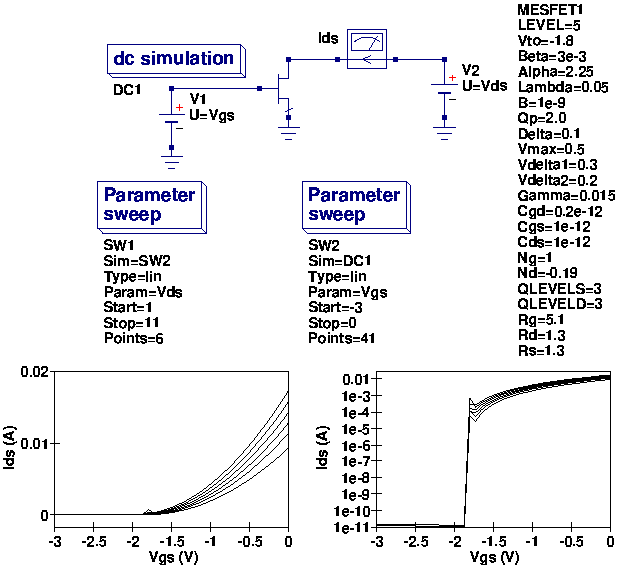
\includegraphics[width=0.9\linewidth]{MESFET_Fig16}  
  \caption{TOM2 LEVEL 5 DC test circuit and Ids-Vgs characteristics} 
  \label{fig:fig16}
\end{figure} 

\begin{figure} 
  \centering
  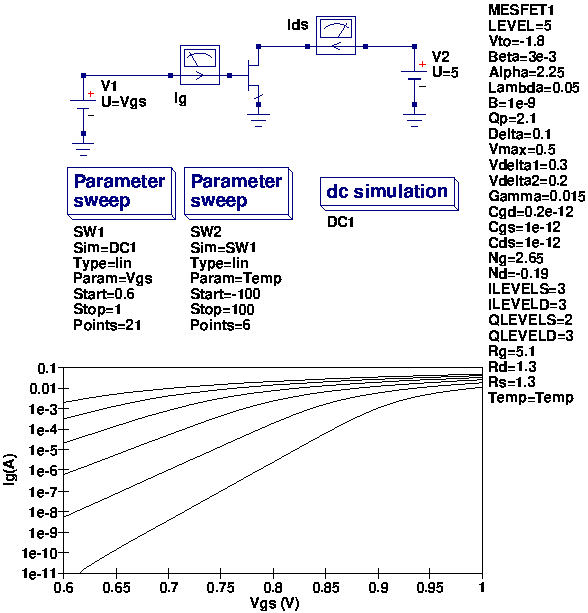
\includegraphics[width=0.9\linewidth]{MESFET_Fig17} 
  \caption{TOM2 LEVEL 5 DC test circuit and Ig-Vgs characteristics} 
  \label{fig:fig17}
\end{figure} 

\begin{figure} 
  \centering
  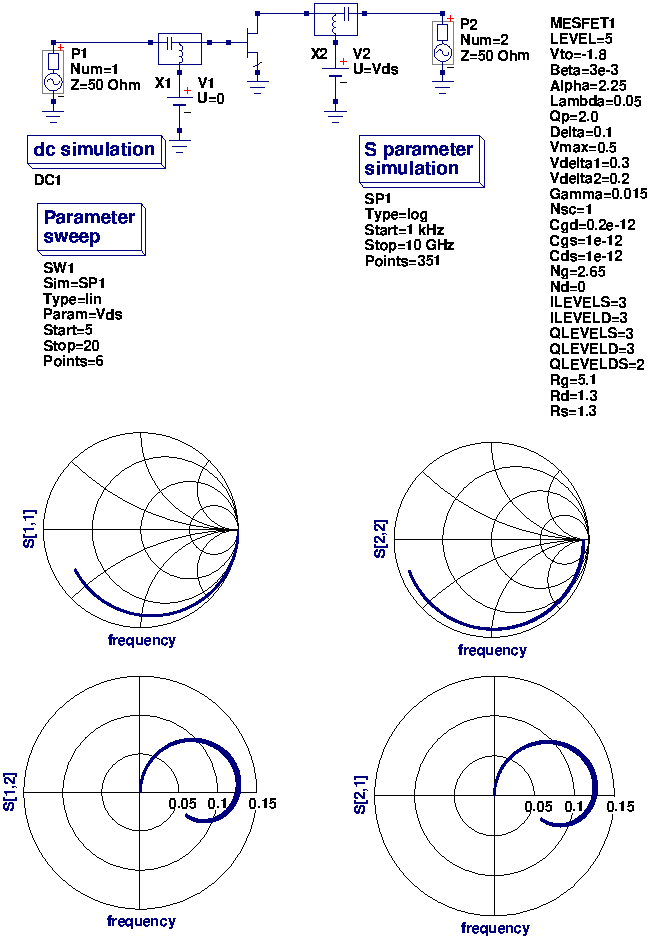
\includegraphics[width=0.9\linewidth]{MESFET_Fig18}  
  \caption{TOM2 LEVEL 5 S parameter test circuit and characteristics} 
  \label{fig:fig18} 
\end{figure} 

\tutsection{Temperature scaling relations}
\begin{verbatim}
T1=Tnom+273.15;
T2=Temp+273.15;
Tr=T2/T1;
con1=pow(Tr, 1.5);
Rg_T2=Rg*(1+Rgtc*(T2-T1));
Rd_T2=Rd*(1+Rdtc*(T2-T1));
Rs_T2=Rs*(1+Rstc*(T2-T1));
Beta_T2=Area*Beta*pow(1.01, Betatc*(T2-T1));
Vt_T2=$vt;
Eg_T1=Eg-7.02e-4*T1*T1/(1108+T1);
Eg_T2=Eg-7.02e-4*T2*T2/(1108+T2);
Vbi_T2=(Tr*Vbi)-(2*Vt_T2*ln(con1)) - ( Tr*Eg_T1-Eg_T2);
Is_T2=Area*Is*pow( Tr, (Xti/N))*limexp(-(`P_Q*Eg_T1)*(1-Tr)/(`P_K*T2));
Cgs_T2=Area*Cgs*(1+M*(400e-6*(T2-T1)-(Vbi_T2-Vbi)/Vbi));
Cgd_T2=Area*Cgd*(1+M*(400e-6*(T2-T1)-(Vbi_T2-Vbi)/Vbi)); 
Vto_T2=Vto+Vtotc*(T2-T1);
Gamma_T2=Gamma*(1+Gammatc*(T2-T1));
Alpha_T2=Alpha*( pow( 1.01, Alphatc*(T2-T1)));
\end{verbatim} 

\tutsection{MESFET noise}

\tutsubsection{Main components}

\begin{itemize}
 \item Thermal noise: generated by resistors Rg, Rd and Rs.
 \item Channel noise: 1. Linear region: essentially thermal noise; 2. Saturation region: diffusion noise.
 \item Gate noise:  Mainly channel noise induced in the gate (via the channel to gate capacitance) The resulting noise is amplified by the MESFET. The capacitive coupling causes the gate noise to have a power spectral density proportional to frequency.
 \item Flicker noise: Due to random carrier generation-recombination in the lattice imperfections or contaminating impurities. Flicker noise power has a $\dfrac{1}{f^{n}}$ behavior, with $n \approx 1.$

\end{itemize}
A typical plot of GaAs MESFET Ids noise current is shown in
Fig.~\ref{fig:fig20}, where the device drain to source noise current
is given by
\begin{equation}
 Idsn = \textrm{channel-thermal-noise-current} + \textrm{flicker-noise-current}
\end{equation}

To a first approximation:
\begin{itemize}
 \item Channel-thermal-noise-current\footnote{Tsivids and Yanis, Operation and modeling of the MOS transistor, McGraw-HIll 1987, p340} = $\sqrt{\dfrac{8 \cdot K \cdot T}{3} \cdot gm \cdot \left\lbrace \dfrac{1+ \alpha + \alpha^{2}}{1+\alpha} \right\rbrace  \cdot Gdsnoi} $


Where $gm = \dfrac{\partial Ids}{\partial Vgs}$,


and  $\alpha = 1 -\dfrac{Vds}{Vgs-Vto}$, when $Vds < \dfrac{3}{Alpha} $ -- Linear region of operation


Or \hspace{1mm}    $\alpha = 0$, when  $ Vds >= \dfrac{3}{Alpha} $ -- Saturation region of operation

\item flicker-noise-current = $\sqrt{\dfrac{Kf \cdot Ids^{Af}}{f}}$

\item Resister thermal noise equations $IRgn = \sqrt{\dfrac{4 \cdot K \cdot T}{Rg}}$ , $IRdn = \sqrt{\dfrac{4 \cdot K \cdot T}{Rd}}$, and
$IRsn = \sqrt{\dfrac{4 \cdot K \cdot T}{Rs}}$
\end{itemize}


\begin{figure} 
  \centering
  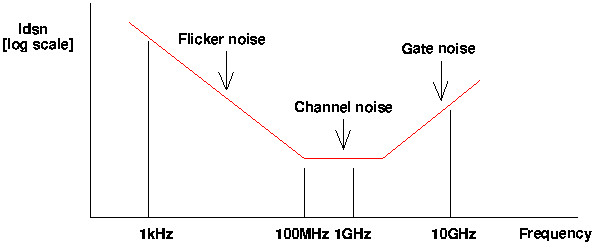
\includegraphics[width=0.9\linewidth]{MESFET_Fig20}  
  \caption{Typical GaAS MESFET Ids noise characteristic} 
  \label{fig:fig20} 
\end{figure} 

\tutsubsection{MESFET equivalent circuit with noise current components}

\begin{figure} [here]
  \centering
  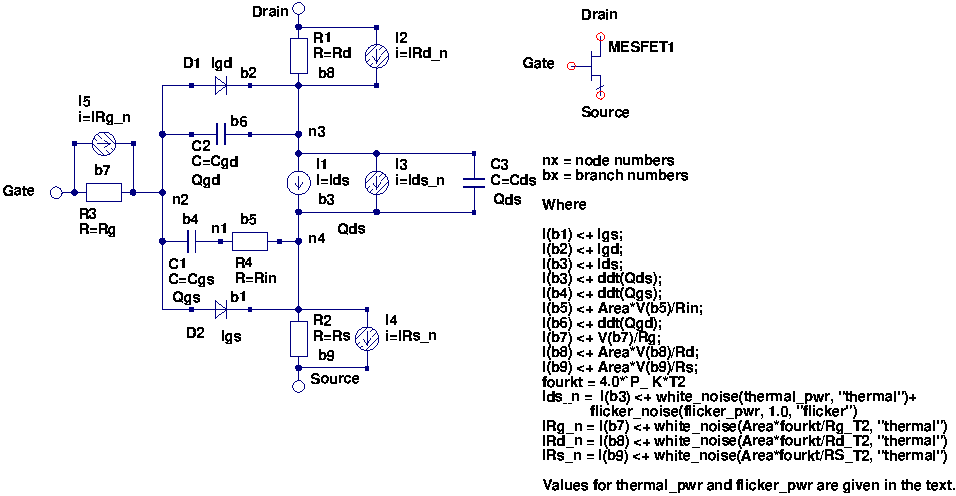
\includegraphics[width=1.1\linewidth]{MESFET_Fig26}  
  \caption{Typical GaAS MESFET equivalent circuit illustrating noise current components} 
  \label{fig:fig26} 
\end{figure} 

\tutsubsection{Curtice hyperbolic tangent model: LEVEL = 1 or 2: Noise equations}
\begin{enumerate}
 \item Verilog-A equations
\begin{verbatim}
fourkt=4.0*`P_K*T2;
gm=2*Beta_T2*(V(b1)-Vto_T2)*(1+Lambda*V(b3))*tanh(Alpha_T2*V(b3));
   if ( V(b3) < 3/Alpha ) begin  An=1-V(b3)/(V(b1)-Vto_T2);
    thermal_pwr= (8*`P_K*T2*gm/3)*((1+An+An*An)/(1+An))*Gdsnoi;
   end
   else
    thermal_pwr=(8*`P_K*T2*gm/3)*Gdsnoi; 
    I(b3)<+white_noise(thermal_pwr,"thermal"); flicker_pwr = Kf*pow(Ids,Af); 
    I(b3)<+flicker_noise(flicker_pwr,1.0,"flicker");
   end
I(b7) <+ white_noise(Area*fourkt/Rg_T2, "thermal");
I(b8) <+ white_noise(Area*fourkt/Rd_T2, "thermal");
I(b9) <+ white_noise(Area*fourkt/Rs_T2, "thermal");
\end{verbatim} 

\item Typical noise simulation results
\begin{figure} [here]
  \centering
  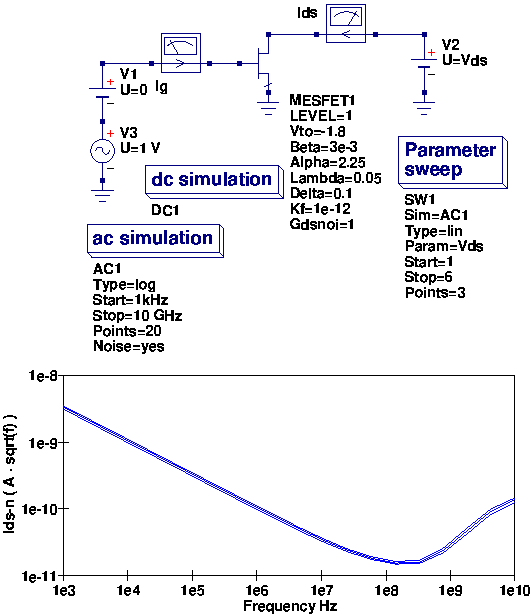
\includegraphics[width=0.8\linewidth]{MESFET_Fig21}  
  \caption{Typical LEVEL 1 (or 2) GaAS MESFET Ids noise characteristic} 
  \label{fig:fig21} 
\end{figure} 

\end{enumerate}

\tutsubsection{Statz \textit{et. al.} (Raytheon) model: LEVEL = 3: Noise equations}
\begin{enumerate}
 \item Verilog-A equations
\begin{verbatim}
if ( V(b3) < 3/Alpha )begin
	H1=(1-(1-(Alpha*V(b3))/3))/(1+B*(V(b1)-Vto_T2));
	gm=2*Beta_T2*(V(b1)-Vto_T2)*(1+Lambda*V(b3))*H1+(Beta_T2*
	   (1+Lambda*V(b3))*pow((V(b1)-Vto_T2),2))*B*H1/(1+B*(V(b1)-Vto_T2));
	An=1-V(b3)/(V(b1)-Vto_T2); 
	thermal_pwr= (8*`P_K*T2*gm/3)*((1+An+An*An)/(1+An))*Gdsnoi;
end
else begin
	gm=2*Beta_T2*(V(b1)-Vto_T2)*(1+Lambda*V(b3))/(1+B*(V(b1)-Vto_T2))+
	(Beta_T2*(1+Lambda*V(b3))*pow((V(b1)-Vto_T2),2))
	*B/pow( (1+B*(V(b1)-Vto_T2)),2);
	thermal_pwr=(8*`P_K*T2*gm/3)*Gdsnoi;
end
I(b3) <+ white_noise(thermal_pwr, "thermal"); 
flicker_pwr = Kf*pow(Ids,Af);
I(b3) <+ flicker_noise(flicker_pwr,1.0, "flicker");
I(b7) <+ white_noise(Area*fourkt/Rg_T2, "thermal");
I(b8) <+ white_noise(Area*fourkt/Rd_T2, "thermal");
I(b9) <+ white_noise(Area*fourkt/Rs_T2, "thermal"); 
\end{verbatim} 

\item Typical noise simulation results
\begin{figure} [here]
  \centering
  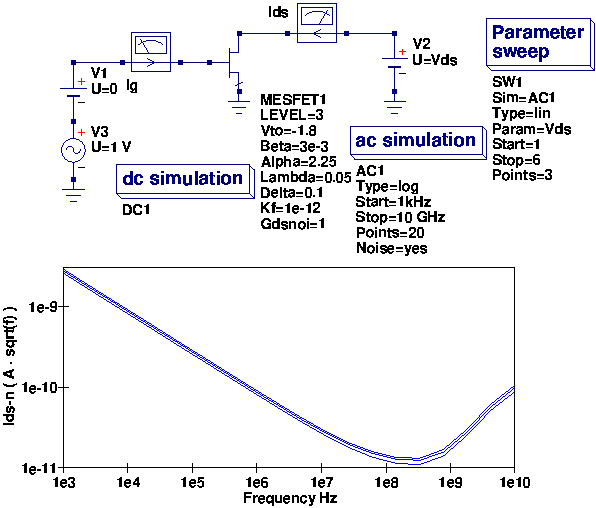
\includegraphics[width=0.8\linewidth]{MESFET_Fig22}  
  \caption{Typical LEVEL 3 GaAS MESFET Ids noise characteristic} 
  \label{fig:fig22} 
\end{figure} 

\end{enumerate}

\tutsubsection{TriQuint Semiconductor TOM 1 model: LEVEL = 4: Noise equations}
\begin{enumerate}
 \item Verilog-A equations
\begin{verbatim}
if ( V(b3) < 3/Alpha )begin
	Ids1=(Beta_T2*pow( (V(b1)-Vto_T2), Qp) )*(1-pow( (1-Alpha*V(b3)/3), 3));
	gm1=Qp*Beta_T2*pow( V(b1)-Vto_T2, Qp-1)*(1-(1-pow(Alpha*V(b3)/3, 3)));
	gm=(gm1*(1+Lambda*V(b3))/(1+Delta*V(b1)*Ids1))*(1+(Delta*V(b3)*Ids1)/
	   (1+Delta*V(b3)*Ids1)); 
        An=1-V(b3)/(V(b1)-Vto_T2); 
	thermal_pwr= (8*`P_K*T2*gm/3)*((1+An+An*An)/(1+An))*Gdsnoi;
end
else begin
	Ids1=(Beta_T2*pow( (V(b1)-Vto_T2), Qp) ); 
	gm1=Qp*Beta_T2*pow( V(b1)-Vto_T2, Qp-1);
	gm=(gm1*(1+Lambda*V(b3))/(1+Delta*V(b1)*Ids1))*(1+(Delta*V(b3)*Ids1)/
	   (1+Delta*V(b3)*Ids1)); 
        thermal_pwr=(8*`P_K*T2*gm/3)*Gdsnoi;
end
I(b3) <+ white_noise(thermal_pwr, "thermal"); 
flicker_pwr = Kf*pow(Ids,Af);
I(b3) <+ flicker_noise(flicker_pwr,1.0, "flicker");
I(b7) <+ white_noise(Area*fourkt/Rg_T2, "thermal");
I(b8) <+ white_noise(Area*fourkt/Rd_T2, "thermal");
I(b9) <+ white_noise(Area*fourkt/Rs_T2, "thermal"); 
\end{verbatim} 

\item Typical noise simulation results
\begin{figure} [here]
  \centering
  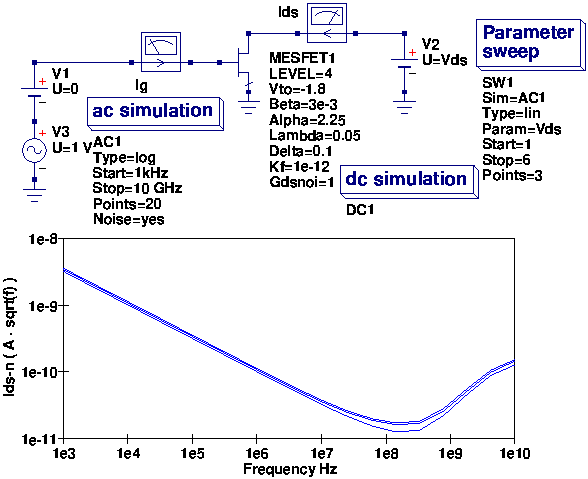
\includegraphics[width=0.8\linewidth]{MESFET_Fig23}  
  \caption{Typical LEVEL 4 GaAS MESFET Ids noise characteristic} 
  \label{fig:fig23} 
\end{figure} 

\end{enumerate}

\tutsubsection{TriQuint Semiconductor TOM 2 model: LEVEL = 5}
\begin{enumerate}
 \item Verilog-A equations
\begin{verbatim}
if ( V(b3) < 3/Alpha )begin
	Nst=Ng+Nd*V(b3);
	if ( Nst < 1.0) Nst=1.0;
	 Vst=Nst*Vt_T2;
	 Vg=Qp*Vst*ln( exp( (V(b1)-Vto_T2+Gamma_T2*V(b3)) / (Qp*Vst) ) + 1);
	 Al= Alpha_T2*V(b3); Fd=Al/sqrt( 1.0+(Al*Al) );
	 Ids1=Beta_T2*pow( Vg, Qp)*Fd;
	 gm1=(Ids1/Vg)*Qp/(exp(-((V(b1)-Vto_T2+Delta*V(b3))/(Qp*Vst)))+1);
	 gm=gm1/pow( (1+Delta*V(b3)*Ids1),2); 
         An=1-V(b3)/(V(b1)-Vto_T2);
 	 thermal_pwr= (8*`P_K*T2*gm/3)*((1+An+An*An)/(1+An))*Gdsnoi;
end
else	begin
	 Nst=Ng+Nd*V(b3); if ( Nst < 1.0) Nst=1.0;
	 Vst=Nst*Vt_T2;
	 Vg=Qp*Vst*ln( exp( (V(b1)-Vto_T2+Gamma_T2*V(b3)) / (Qp*Vst) ) + 1);
	 Al= Alpha_T2*V(b3); Fd=Al/sqrt( 1.0+(Al*Al) );
	 Ids1=Beta_T2*pow( Vg, Qp)*Fd;
	 gm1=(Ids1/Vg)*Qp/(exp(-((V(b1)-Vto_T2+Delta*V(b3))/(Qp*Vst)))+1);
	 gm=gm1/pow( (1+Delta*V(b3)*Ids1),2);
	 thermal_pwr=(8*`P_K*T2*gm/3)*Gdsnoi;
end
I(b3) <+ white_noise(thermal_pwr, "thermal"); 
flicker_pwr = Kf*pow(Ids,Af);
I(b3) <+ flicker_noise(flicker_pwr,1.0, "flicker");
I(b7) <+ white_noise(Area*fourkt/Rg_T2, "thermal");
I(b8) <+ white_noise(Area*fourkt/Rd_T2, "thermal");
I(b9) <+ white_noise(Area*fourkt/Rs_T2, "thermal"); 
\end{verbatim} 

\item Typical noise simulation results
\begin{figure} [here]
  \centering
  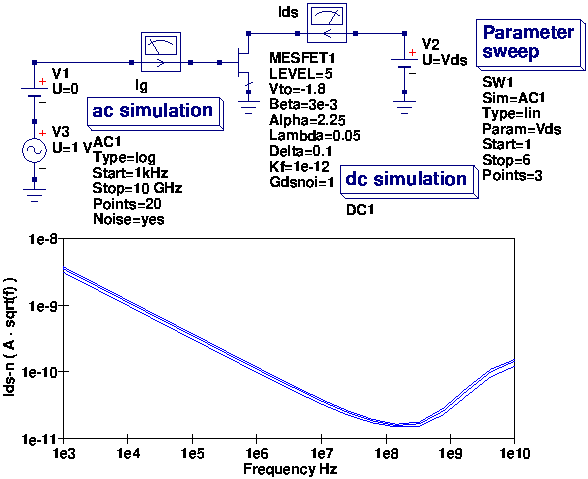
\includegraphics[width=0.8\linewidth]{MESFET_Fig24}  
  \caption{Typical LEVEL 5 GaAS MESFET Ids noise characteristic}  
  \label{fig:fig24} 
\end{figure} 

\end{enumerate}

\tutsection{Adding external passive components to the MESFET models}

The Curtice model outlined in the first Qucs report on MESFETs
included lead inductance in each of the device signal paths. These
inductances were not included in the Verilog-A models described in
this report, mainly to simplify the model code.  If required they can
be added as external components.  The test circuit shown in
Fig.~\ref{fig:fig25} indicates how this can be done and illustrates
the effect such components have on the Curtice S parameter
characteristics.

\begin{figure}  
  \centering
  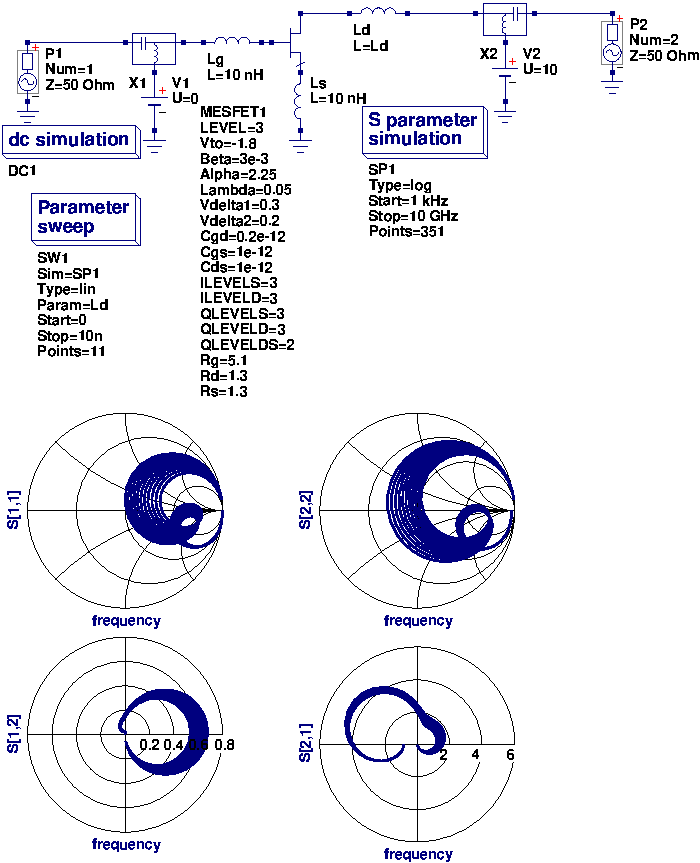
\includegraphics[width=0.9\linewidth]{MESFET_Fig25}  
  \caption{S parameter simulated characteristics for test circuit shown in Fig.~\ref{fig:fig5} that has external inductance added}  
  \label{fig:fig25} 
\end{figure} 


\tutsection{End note}

MESFETs are important high frequency devices which have been missing
from the range of active component models supplied with Qucs.  While
developing the models described in this report I have attempted to
make them as flexible as possible so as to allow users the opportunity
to select which model, or indeed the make-up of the components of a
model, they would like to try for a specific simulation.  The work
described in this report is very much work in progress, mainly because
there are a number of other published MESFET models that have not been
included.  My intention has simply been to provide a number of
practical models which were not previously available to Qucs users.
Also knowing that many Qucs users have an interest in high frequency
circuit design and simulation, the work would be of direct relevance
to making Qucs more ``universal``. The procedures employed for model
development are another example of the work being undertaken by the
Qucs team in response to Qucs being adopted by the wider modelling
community as part of the Verilog-A compact device standardization
project. Overall the simulation results from the models described here
show a high degree of consistency from DC to the high frequency S
parameter domain. The noise results are particularly interesting as
they are based on mix of available theories and extensions introduced
especially for Qucs.  Some readers will probably have spotted one area
where there appears to be differences in the simulation results from
the different models; look at the S[1,2] and S[2,1] characterstics for
each model.  Here there are noticeable difference which are possibly
due to the lack of symmetry in some of the model charge equations?
MESFET modelling is a complex subject, suggesting that there are
likely to be errors /bugs in the models.  If you find an error/bug
please inform the Qucs development team so that we can correct
problems as they are found. In the future, particularly if the
response to this group of models is positive, I will attempt to add
more MESFET models to Qucs. Once again a special thanks to Stefan Jahn
for all his help and encouragement over the period that I have been
developing the Qucs MESFET models and writing the report which
outlines their physical and mathematical fundamentals.
